\chapter{Fitting a model to the data}\label{ap:prob_theory}

% \subsubsection{Foundational knowledge on probability theory}
\section{The Gaussian distribution}

\begin{wrapfigure}{r}{.5\textwidth}
    \centering
    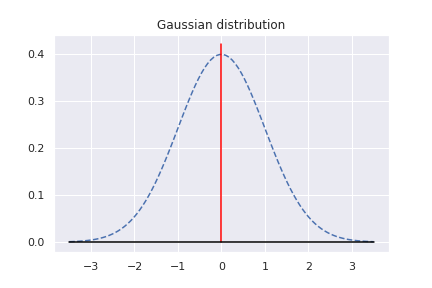
\includegraphics[width=\linewidth]{figs/normal_dist.png}
    \caption[The probability density function for a standard Gaussian or normal distribution]{\small \textbf{The probability density function for a standard Gaussian or normal distribution.}}
    \label{fig:gauss}
\end{wrapfigure}


Let's say we observe a random variable $x$. Random variables have a value that is not predetermined, but sometimes we know how the probability of drawing a random value is depending on that value. When the random number can assume any number (i.e. not only discrete integers), then a probability density function gives the probability density for the support of $\mathcal{X}$ (i.e. the values that $x$ can assume). One well-known example of such a probability density function is the Gaussian distribution. It is defined by \ref{eq:gauss}.

\begin{equation}\label{eq:gauss}
    \mathcal{N}(x|\mu, \sigma^2)=\frac{1}{(2 \pi \sigma ^2)^{\frac{1}{2}}} e^{- \frac{1}{2\sigma ^2}(x - \mu)^2}
\end{equation}

The mean $\mu$ is the value around which all drawn samples are centered, and the standard deviation $\sigma$ tells us how far the drawn samples are spread out from this point. Drawing a sample of $n$ independent and identically distributed (i.i.d.) data points from the Gaussian distribution given its mean and variance is done with a probability of the product of the probabilities of drawing the individual data points (see \ref{eq:gauss_prod}, where $\textbf{x}^n$ is a set of $n$ data points).

\begin{equation}\label{eq:gauss_prod}
    p(\textbf{x}^n | \mu, \sigma^2) = \prod_{i=1}^{n}{\mathcal{N}(x_i|\mu, \sigma^2)}
\end{equation}

Sometimes, we deal with multivariate random variables. In this case, every data-point $\bm{x}_i$ and the mean $\bm{\mu}$ are $d$-dimensional vectors and the covariance matrix $\bm{\Sigma}$ is a $d \times d$ matrix noting the co-variances among all dimensions. In this case, $\textbf{X}$ is a matrix containing $n$ rows $\textbf{x}_i$ of length $d$ for each data point. In this case, $\bm{\mu}^d$ is a $d$-dimensional vector where $\mu_j$ notes the mean of the $j$th variable. The covariances between all variables are given by positive semi-definite matrix $\bm{\Sigma}$, where $\bm{\Sigma}_{i,j}$ describes the covariance between the $i^\text{th}$ and $j^\text{th}$ variable. Note that $\bm{\Sigma}$ is symmetric, as a property of covariance, and that $\bm{\Sigma}_{i,i}=cov(x_i,x_i) = var(x_i)$. For a set of independent variables, $\bm{\Sigma}$ is a diagonal matrix, since the $cov(x_i,x_j)$ is $0$ when $i\neq i$. In a multivariate setting, the Gaussian distribution takes the form of \ref{eq:gaus_mn}.

\begin{equation}\label{eq:gaus_mn}
    \mathcal{N}(\textbf{x}|\bm{\mu}, \bm{\Sigma})=\frac{1}{(2 \pi)^{\frac{m}{2}}}\frac{1}{|\bm{\Sigma}|^{\frac{1}{2}}} e^{- \frac{1}{2}(\textbf{x} - \bm{\mu})^T \bm{\Sigma}^{-1}(\textbf{x} - \bm{\mu})}
\end{equation}

\section{Likelihood and the posterior}
 Let's say we have the probability density function of $\bm{x}$, $p(\bm{x}|\theta)$, where $\theta$ holds the parameters of the distribution of $p(x)$ (e.g. in this case $\theta = (\mu, \sigma^2)$). Apart from deriving the probability of drawing a value from a given distribution and its parameters, we can also derive the likelihood of the parameters of the distribution being certain values given only the observed data. A noteworthy difference between the probability and the likelihood is that the probability necessarily sums up to $1$ when integrated over the support of $\mathcal{X}$, but the likelihood does not when integrating over the parameter space of $\theta$. The likelihood is given by $\mathcal{L}(\theta|\bm{x}) = p(\bm{x}|\theta)$. This likelihood is often given by its logarithm, known as the log-likelihood. On the one hand, this makes mathematical manipulations with Gaussian distributions a lot easier. On the other hand, the log function converts very small numbers to larger ones, which helps to avoid numerical underflow on electronic devices. Converting the likelihood function of \ref{eq:gauss_prod} to a corresponding log-likelihood function results in \ref{eq:logprob} (derivation in \ref{AP:log_prob}).

\begin{equation}\label{eq:logprob}
    \ln \mathcal{L}(\mu, \sigma^2 | \bm{x}) = \ln p(\textbf{x} | \mu, \sigma^2) = -\frac{n}{2} \ln 2 \pi -\frac{n}{2} \ln \sigma ^2 - \frac{1}{2\sigma ^2} \sum_{i=1}^{n} (x_i - \mu)^2
\end{equation}

Using the log-likelihood has two advantages: It makes mathematical manipulations to the distribution fairly easy and it avoids numerical underflow errors by converting very small numbers to larger ones. Since the log function is monotonically increasing, the maximum of the likelihood function s found for the same value as the maximum of the log-likelihood.

 The likelihood, however, is not the same as the probability that $\theta$ is responsible for generating data $\bm{x}$. According to Bayes' theorem, $p(A|B) = \frac{p(B|A) p(A)}{p(B)}$, and therefore the likelihood of parameters $\theta$ being responsible for observed data $\bm{x}$ is given by $p(\theta|\bm{x}) = \frac{p(\bm{x}|\theta) p(\theta)}{p(\bm{x})}$. In this construction, the first term $P(\bm{x}|\theta)$ is the likelihood and the second term $p(\theta)$ is known as the prior. The prior takes the distribution of the parameters into account. Since the divisor is not dependent on $\theta$, $p(\bm{x}|\theta) p(\theta) \propto p(\theta|\bm{x})$ so that the product of the prior and likelihood determines the probability of $\theta$ being a certain value given the data. The last term, $p(\bm{x})$, is known as the evidence. It normalizes the probability, so that the posterior integrated over the parameter-space $\theta$ sums to $1$. When estimating $\theta$ given $\bm{x}$, a point estimate is given by $\text{argmax}_\theta p(\theta|\bm{x})$.
 
 Often, a prior distribution of $\theta$ is unknown or assumed to be of a uniform shape. In this case, the prior $p(\theta$ is a constant that is non-dependent on $\theta$ and $ p(\theta|\bm{x}) \propto p(\bm{x}|\theta)$. The point estimate for $\theta$ is then $\text{argmax}_\theta p(\bm{x}|\theta)$, known as the maximum likelihood (\textbf{ML}) estimate. This estimate can be found by taking the derivative of $\mathcal{L}(\theta|\bm{x})$ and setting it to $0$. For example, the ML estimates for $\mu$ is given by $\mu_{ML} = \frac{1}{n} \sum_{i=1}^{n} x_i$ and for $\sigma^2$ by $\sigma^2_{ML} = \frac{1}{n} \sum_{i=1}^{n} (x_i - \mu_{ML})^2$ (see \ref{AP:mu_ML} and \ref{AP:s2_ML}).\\

\section{Gaussian mixture models and EM}\label{app:gmm_em}
Now imagine that our data-set consists of different `groups' that all have their own mean and covariance matrix. For example, we may have a data-set with several cell-types, and every cell-type demonstrates their own pattern of gene expression. If our data-set consists of $K$ different Gaussians, then we have a Gaussian mixture model (\textbf{GMM}), of which the probability density function is denoted by \ref{eq:mm}.

\begin{equation}\label{eq:mm}
    p(x) = \sum_{k=1}^K \pi_k \mathcal{N}(x|\bm{\mu}_k, \bm{\Sigma}_k)
\end{equation}

In this example, $\bm{\mu}_k$ and $\bm{\Sigma}_k$ give the means and covariance matrix of each distribution $k$ and $\pi_k$ is the proportion in which mixture component $k$ is responsible for generating the data-set, such that $\sum^K_{k=1}\pi_k = 1$ and $\pi_k\geq0$ for all $k$.
 Finding the set of parameters $\theta = (\pi, \bm{\mu}, \bm{\Sigma})$ in this scenario is not as straight forward as the ML approach we saw earlier. To approximate $\theta$ for this model, we can use an iterative expectation-maximization (\textbf{EM}) algorithm. An EM-algorithm consist of two steps:
 
 \begin{itemize}
     \item In the Expectation-step, the expected log-likelihood function of the complete data-set (observed data and missing parameters) is estimated from their joint probabilities.
     \item In the maximization step, the parameters $\theta$ are maximized based on the estimated log-likelihood.
 \end{itemize}

 After we have chosen some arbitrary initial values for $\bm{\mu}_k$, $\bm{\Sigma}_k$ and $\pi_k$, we start with the E-step. In the E-step of our algorithm, we try to find the complete log-likelihood function. Let $\bm{z}_i$ denote which mixture component has generated data-point $i$. Then the complete likelihood function is given by \ref{eq:gmm_llh}, where $\mathbb{I}[z_i=j]$ evaluates to $1$ if true and $0$ otherwise. 

\begin{equation}\label{eq:gmm_llh}
    \mathcal{L}(\bm{X}|\theta, \bm{z}) = \prod^n_{i=1} \prod^K_{j=1} \mathcal{N}(\bm{x}_i|\theta_k)^{\mathbb{I}[z_i=j]}
\end{equation}

Now, $\bm{z}$ (i.e. which data-points were generated by which distribution) is unknown, but instead of $\mathbb{I}[z_i=j]$, we could use the probability $p(z_i=j)$. We know that $p(\bm{x}_i|z_i=j) = \mathcal{N}(\bm{x}_i|\bm{\mu}_j, \bm{\Sigma}_j)$ and therefore, we can compute the posterior $p(z_i=j|\bm{X})$ according to Bayes' theorem as done in \ref{eq:mix_prob}.

\begin{equation}\label{eq:mix_prob}
    p(z_k=j|\textbf{x}_i)
    =\frac{p(z_i=1) p(\textbf{x}_i|z_i=j)}{\sum^K_{k=1}p(z_i=k)p(\textbf{x}_i|z_i=k)}
    = \frac{\pi_j\mathcal{N}(\textbf{x}_i|\bm{\mu}_j, \bm{\Sigma}_j)}{\sum_{k=1}^K\pi_k\mathcal{N}(\textbf{x}_i|\bm{\mu}_k, \bm{\Sigma}_k)} 
\end{equation}

In the literature, the posterior probability is often denoted as $\gamma(z_{k,i}) = p(z_i=k|\bm{X})$.
With this, we can compute the expected complete log-likelihood $\ln \mathcal{L}(\theta|\bm{X}) = \sum^n_{i=1} \sum^K_{j=1} p(z_i=j) \ln \mathcal{N}(\bm{x}_i|\theta_k)$. In the M-step, we utilise this expected log likelihood to calculate ML-estimates for the mean $\bm{\mu}_k$, covariance-matrix $\bm{\Sigma}_k$ and mixing coefficient $\pi_k$ of each distribution $k$.

We start off with the mean of each distribution $k$. Setting the derivative with respect to $\bm{\mu}_k$ to $0$ shows that the ML estimate is simply given as the weighted average of all points belonging to distribution $k$ (\ref{eq:mm_mu}.

\begin{equation}\label{eq:mm_mu}
    \bm{\mu}_k = \frac{1}{\sum^n_{i=1} \gamma(z_{k,i})} \sum^n_{i=1} \gamma(z_{k,i}) \textbf{x}^m_i
\end{equation}

Similarly, the variance is computed as the weighted variance.

\begin{equation}\label{eq:mm_var}
    \bm{\Sigma}_k = \frac{1}{\sum^n_{i=1} \gamma(z_{k,i})} \sum^n_{i=1} \gamma(z_{k,i}) (\textbf{x}^m_i-\bm{\mu}_k)(\textbf{x}^m_i-\bm{\mu}_k)^T
\end{equation}

Finally, $\pi_k$ is obtained as the average of the individual probabilities with which points belong to distribution $k$.

\begin{equation}\label{eq:mm_mix}
    \pi_k = \frac{\sum^n_{i=1}{} \gamma(z_{k,i})}{n}
\end{equation}

Having obtained new values for all relevant parameters, we return to the E-step and obtain new posterior probabilities. The process is repeated until a converged state is reached.\\
